\documentclass{Paper}
\usepackage{tikz}
\usepackage{float}
\usetikzlibrary{graphs, positioning, quotes, shapes.geometric}
\articletitle{神奇的动植物——蚰蜒}
\name{中国古代博物学233-6组}
\begin{document}
\makeheader
\tableofcontents
\newpage
\section{初识蚰蜒}
2024年7月14日晚,于法喜寺旁发现了蚰蜒,其奇特的外观以及外号引起了我们的注意。

蚰蜒体短而微扁,棕黄色,体长1-6厘米,主要由头部及毒牙、触角、背板、腹板、15对步足和内脏团等部分组成。
头部两侧对称生长着由大量单眼组成的伪复眼。头部最前端生有两根触角。它的身体共有15节腹板,相邻两节之间上下重叠,以鱼鳞状排列。
背板也呈分节结构,同样以鱼鳞状排列。全身每节都长有一对细长的步足。

\begin{figure}[H]
    \centering
    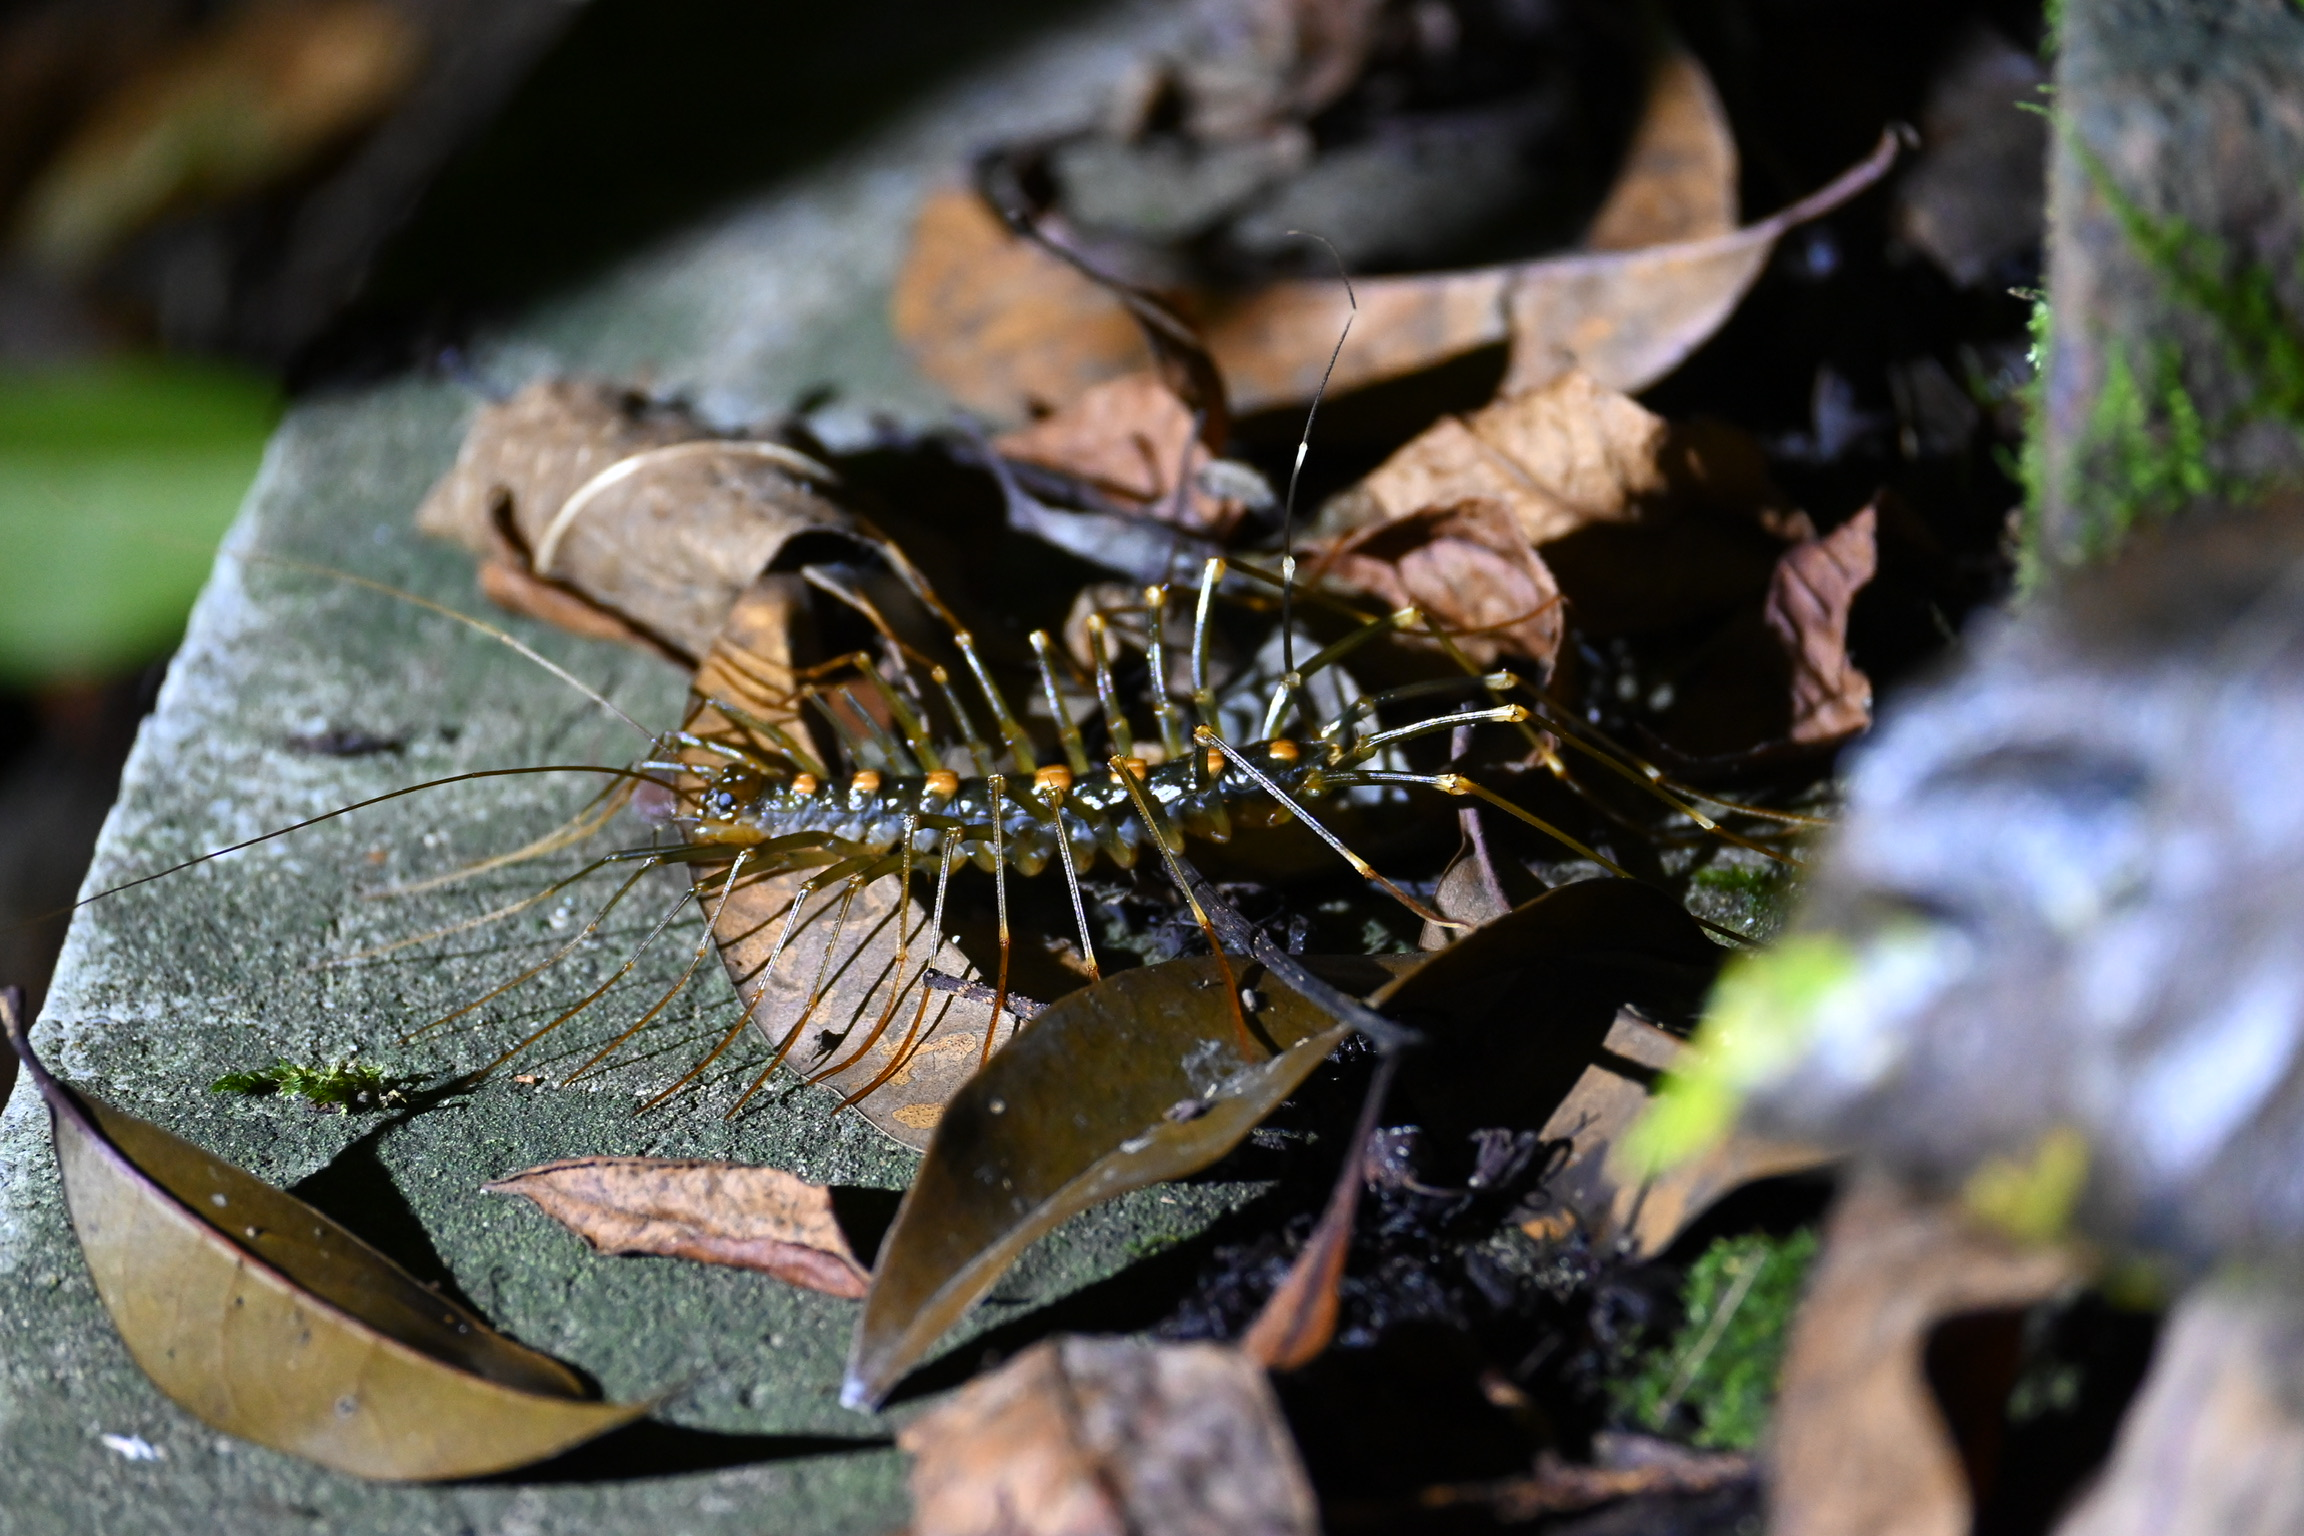
\includegraphics[width = .8\textwidth]{../assets/微信图片_20250226160858.jpg}
    \caption{拍摄到的蚰蜒图片}
\end{figure}
\section{生态地位}
蚰蜒具有许多有益于环境的作用,是环境中必不可少的昆虫之一。
\subsection{控制害虫}
蚰蜒主要以蜘蛛、蚊子、蠕虫等小型昆虫为食,可帮助人类消灭毒虫、蠹虫、苍蝇等害虫,可控制这些害虫的繁殖,可以维持家中环境卫生以及在园艺等领域减少害虫的影响。
\subsection{生态系统中的地位}
蚰蜒是生态系统中其他捕食者的食物,例如鸟类、爬行动物和哺乳动物。蚰蜒的虫卵和幼崽容易被捕食,是食物链中的一环,有利于维持生态系统稳定。
\subsection{分解有机物}
蚰蜒能够帮助分解死亡的植物和动物组织,保持土壤的肥沃。
\subsection{改善土壤结构}
它们的活动有助于土壤的通气和排水,保持土壤的健康。
\section{文化象征}
\subsection{阴湿污秽之物}
蚰蜒常出没于阴暗潮湿的墙角、朽木或废墟,其存在被视为环境脏乱、家宅不宁的征兆。
\begin{enumerate}
    \item 如清代《燕京岁时记》 载:``蚰蜒上墙,家宅必败'',民间建房时甚至刻意用石灰涂抹墙缝以驱虫辟秽。

    《燕京岁时记》是清代一部详细记录北京(旧称``燕京'')岁时节令、民俗风物的笔记体著作,
    由满族文人富察敦崇(字礼臣)于光绪三十二年(1906年)编纂成书。
    全书以农历时序为纲,按月分述北京地区的节日习俗、物产饮食、民间信仰及市井生活,是研究晚清北京民俗文化的重要文献。

    \item 《九思·哀岁》巷有兮蚰蜒,邑多兮螳螂 。(最早的出处)

    这句话的翻译是:``街巷之中潮虫遍地,城镇之上充斥螳螂。 ''

    \item 《榆社县志》二月一日,各家用灰围住房子,煮芥菜来驱赶蚰蜒。东人呼皆今蚰蜒,喜入耳者也。
\end{enumerate}

\subsection{讽刺之用}

\begin{enumerate}
    \item 《聊斋志异》卷十一 第15《蚰蜒》:``学使朱矞三家门限下有蚰蜒,长数尺。每遇风雨即出,盘旋地上如白练然。按蚰蜒形若蜈蚣,昼不能见,夜则出,闻腥辄集。或云:``蜈蚣无目而多贪也''

    文中``学使朱矞三''即朱雯,字三,石门(今浙江桐乡市)人。康熙三年(1664)二甲第三十名进士,历官孝感知县、江宁同知。康熙三十年(1691)以山东按察司副使提督全省学政,迁济东道。蒲松龄对朱雯颇有微词,在此文中指名道姓,将其比作蚰蜒(形类蜈蚣),讽刺他``无目多贪''``闻腥辄集'',可谓辛辣至极。

    \item 《法华义疏\footnote{佛教词典}》记载:``重嗔如蚖蛇蝮蝎,轻嗔如蜈蚣蚰蜒。
\end{enumerate}

\subsection{经济生活的双面符号}

\begin{enumerate}
    \item 吉兆:北方部分地区称蚰蜒为``钱串子'',认为其出现预示财富积累(因形似串起的铜钱),山西某些地区甚至忌杀蚰蜒,以免``断了财路''。
    \item 凶兆:江南民间则认为蚰蜒是``破财虫'',若爬过钱柜或账本,需立即焚香驱赶,以防家财流失。
\end{enumerate}

\subsection{纠缠与琐碎之事的隐喻}

红楼梦中有如下场景:《红楼梦》第三九回:那焙茗去后,宝玉左等也不来,右等也不来,急的热地里的蚰蜒似的。

\subsection{指曲折蜿蜒}

\begin{enumerate}
    \item 造字法
    \item 老人``蚰蜒路''的说法
\end{enumerate}
\section{社会习俗}
\subsection{``蚰蜒卦''与占卜}

明代《五杂俎》载,某些地区通过观察蚰蜒爬行轨迹占卜(称``蚰蜒卦''),但其法已失传,仅存``虫迹如谶''的模糊记载。

关于《五杂俎》:《五杂俎》是明代谢肇淛创作的一部著名的随笔札记。
内容包括读书心得和事理的分析,也记载政局时事和风土人情,涉及社会和人的各个方面。

\subsection{入耳禁忌}
入耳禁忌是指古人认为蚰蜒进入耳朵后会导致出现头痛、疯癫等症状

明·陆容《菽园杂记》:北方有虫名蚰蜒,状类蜈蚣而细,好入人耳。
闻之同僚张大器云:人有蚰蜒入耳不能出,初无所苦,久之觉脑痛。疑其入脑,甚苦之,而莫能为计也。
一日将午饭,枕案而睡,适有鸡肉一盘在旁,梦中忽喷嚏,觉有物出鼻中,视之,乃蚰蜒在鸡肉上,自此脑痛不复作矣。
又同僚苏文简在山海关时,蚰蜒入其仆耳。
文简知鸡能引出,急炒鸡置其耳旁,少顷,觉有声鍧然。乃此虫跃出也。

关于《菽园杂记》:此书对明代朝野故实叙述颇详,而且较少抄袭旧文,论史事、叙掌故、谈韵书、说文字,皆大多为自己的见解,
被他同时代的王鏊称为明朝记事书第一。
\section{中外文化对比}
\subsection{日本:妖怪与家族象征}
在日本民间传说中,蚰蜒(ゲジ)被视为``家付き神''(家宅精灵)的化身,既能护宅亦能作祟。传说百足蚰蜒修炼千年可化身为``女郎蜘蛛'',象征执念与贪欲。
\begin{figure}[H]
    \centering
    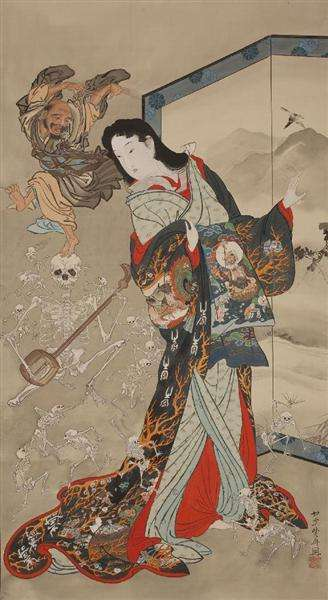
\includegraphics[width = .4\textwidth]{../assets/1.0/图一:河锅晓斋《地狱太夫图》.jpg}
    \caption{河锅晓斋所绘《地狱太夫图》}
\end{figure}

\subsection{欧洲:无害的``屋虫''}
西方文化中,蚰蜒被视为清除蚊虫的益虫,无强烈文化寓意。但因其外形可怖,维多利亚时期小说常以蚰蜒爬过尸体渲染恐怖氛围。
\end{document}